\section{Design of CryptDB}
\label{s:design}


\begin{figure}[t!]
\centering
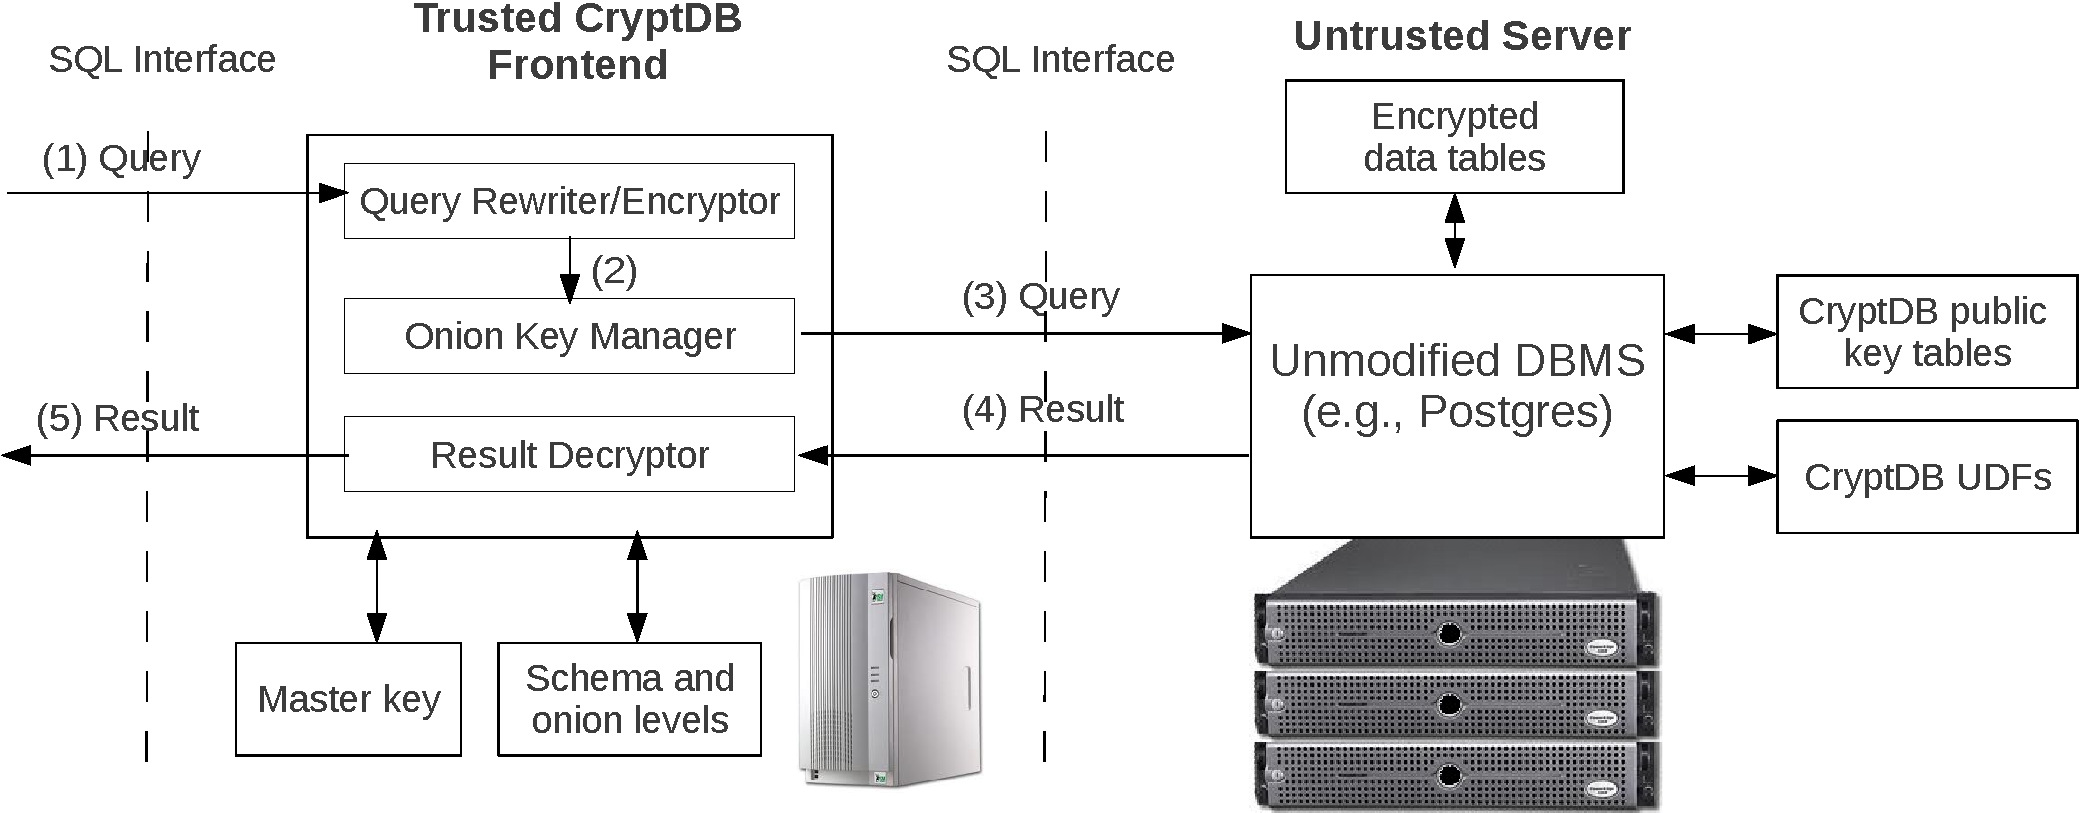
\includegraphics[width=3.45in]{fig/systemoverview.pdf}
\caption{System overview.
    Steps (1)-(5) illustrate typical query flow, with the user or
    application issuing query (1) and receiving result (5).
    UDF stands for user-defined function.}
\label{fig:architecture}
\end{figure}


CryptDB works by allowing the DBMS server to execute SQL queries
on encrypted data almost as if it were executing the same queries
on plain-text data.  In CryptDB, the query plan for an encrypted
query remains the same as for the original query, but individual
operations comprising the query, such as equality comparison or
summation, are performed on ciphertexts, and use modified operators
in some cases.

Figure~\ref{fig:architecture} shows the architecture of CryptDB\@.
\name{} is composed of two parts: a trusted client-side \textit{frontend},
and an untrusted DBMS {\em server}.  The frontend keeps track of a secret
master key $\MK$, the database schema as seen by the application (i.e.,
without encryption), and the level of onion encryption currently exposed
at the server for each data item.  The server, on the other hand,
keeps track of the encrypted schema, the encrypted versions of user data
(i.e., the lowest level of encryption revealed to the server by the
frontend), and auxiliary tables used by CryptDB\@.  The server implements
CryptDB-specific UDFs that enable the
frontend to compute on ciphertexts on the server.  Finally, the server
stores encrypted versions of the frontend's state, including the schema
and the current onion levels, in a separate table, encrypted with $\MK$,
which allows frontends on multiple client machines to synchronize with
one another.

% \nz{Distributed front-end synchronization?  Basically master key, schema,
% and onion levels.  Use transactions to serialize onion level changes.}

Figure~\ref{fig:architecture} also illustrates the typical flow of a query
in CryptDB\@.
In step (1), the user issues a query, which is first passed through the query
rewriter/encryptor (QRE)\@. This module anonymizes each table and column name.
Using the master key $\MK$, this module encrypts each constant in the query with
an encryption scheme allowing the desired operation, as we will describe shortly.
In step (2), the query is passed to the onion key manager (OKM)\@. This module
assesses if the server should be given onion keys to execute the
query. If so, the OKM provides the necessary onion keys by issuing an
\texttt{UPDATE} query at the server that invokes a UDF to adjust the security
of the appropriate columns to increase their functionality. In step (3), the OKM
forwards the anonymized query to the server, which executes it using standard SQL
(and occasionally invokes more UDFs, as we will explain). In step (4), the DBMS
returns the query result, and in step (5) the result decryptor (RD) decrypts the
results and returns them to the user. We elaborate on these steps in the rest
of this section.





\subsection{SQL-aware Encryption Strategy}

To implement encryption that allows SQL query processing, we use existing
encryption schemes, optimize a recent scheme, and design a new
cryptographic primitive for joins, as we will now describe.
CryptDB uses the same level of encryption to encrypt all data items in
a given column, so that the same computation can be performed on every
element in that column.

For each encryption type, we explain the security property that CryptDB requires
from it. We explain how to implement it with tools that are believed to achieve such
security; if such tools are ever broken, they can be replaced with other tools
that provide such property, without breaking the security design of CryptDB\@.
 
\textbf{Random} ($\RND$)\@. $\RND$ provides maximum privacy, such as
indistinguishability under an adaptive chosen-ciphertext attack (IND-CCA2),
also known as semantic security.
In particular, two equal values will be mapped to different encryptions with
high probability. $\RND$ does not allow any computation to be performed efficiently on the
ciphertext.  To implement $\RND$, we use AES in UFE mode~\cite{desai:ufe}.

\textbf{Deterministic} ($\DET$)\@. $\DET$ has a slightly weaker guarantee:
it only leaks which encrypted values correspond to the same data value, and
nothing else. This encryption level allows the server to perform equality
checks, which means it can perform selects with equality filters, equality
joins, GROUP BY, COUNT, DISTINCT, etc.
There are many ways to implement $\DET$, such as
$\DET_K(v)=\RND_{K_1}(v) ~ \| ~ \mathsf{HMAC}\mathrm{-}\mathsf{SHA1}_{K_2}(v)$,
where $\|$ is the concatenation operator, $K_1$ and $K_2$ are two keys derived
from $K$, and $K$ itself is derived by encrypting the table and column names
with $\MK$\@.
For this $\DET$ construction, the server compares two encryptions by
comparing their $\mathsf{HMAC}\mathrm{-}\mathsf{SHA1}$ values.
% We implement $\DET$ using AES in counter mode with a
% separate IV (counter value) for each column, derived by encrypting the table
% and column names with $\MK$\@.

\textbf{Order-preserving encryption} ($\OPE$)\@. $\OPE$ allows order relations
between data items to be established based on their encrypted values, but does
not leak any other information about the data content. A recent proposal for
$\OPE$~\cite{boldyreva-ope} is an encryption scheme that preserves order:
if $x < y$, then $\OPE_K(x) < \OPE_K(y)$, for any secret key $K$\@.
Therefore, if a column is encrypted with $\OPE$, the
server can perform range queries when given encrypted constants
$\OPE_K(c_1)$ and $\OPE_K(c_2)$ denoting the range $c_1$ through $c_2$.
Moreover, the server can perform ORDER BY, MIN, MAX, SORT, etc.

$\OPE$ is a weaker encryption scheme because it reveals order.  Thus, the
frontend will only reveal $\OPE$-encrypted columns to the server if users
request range queries on those columns. $\OPE$ has provable security
guarantees: the encryption is equivalent to a random permutation that
preserves order.  Therefore, the difference between two encryptions
$\OPE_K(y) - \OPE_K(x)$ is basically random, and is not equal to $y - x$
except for the sign.

A provably secure $\OPE$ scheme was only proposed last
year~\cite{boldyreva-ope}.  There was no implementation of the scheme,
or any measure of how practical it would be, so we implemented it.
The initial performance was about $20$ ms per encryption, which was not great,
given that each row in a table may have a few items that should be encrypted
with $\OPE$\@.  We implemented several optimizations to reduce the cost of $\OPE$\@.
At a high-level, given a value $v$, $\OPE$ performs binary search in the field
of encryptions to find an encryption for $v$.  We realized that intermediate
search results can be reused across encryptions of different values, so we
cache them when performing many such encryptions (e.g., upon database load).
To search the cache efficiently we used fast AVL binary search trees.  This
reduced the cost of $\OPE$ encryption to $4$ ms, without affecting its security.
We also implemented a hypergeometric sampler that lies at the core of $\OPE$\@.
The most efficient such scheme was proposed in $1988$ (now used in many tools
such as MathWorks)~\cite{HGD88}, and we translated its original implementation
from Fortran-1988.


\textbf{Homomorphic encryption} ($\HOM$)\@. $\HOM$ is an encryption scheme
that is IND-CCA secure, but allows the server to perform computations on
encrypted data, the final result being decrypted by the frontend. While
homomorphic encryption for general operations is prohibitively
slow~\cite{trillion}, homomorphic encryption for summation is efficient.
To support summation, we implemented the Paillier cryptosystem~\cite{Paillier99}.
With Paillier, multiplying the
encryptions of two values results in an encryption of the sum of the values,
i.e., $\HOM_K(x) \cdot \HOM_K(y) = \HOM_K(x+y)$, where multiplication is
performed modulo some public-key value.  When the server performs summation
on a column encrypted with $\HOM$,
it calls a UDF that performs Paillier multiplication, and uses CryptDB's
public key table to look up $K$, to homomorphically compute a ciphertext
corresponding to the sum of the plaintext values.  $\HOM$ is secure under
a chosen-plaintext attack.  $\HOM$ can also be used for computing averages
(by having the server return the sum and the count, and dividing the decrypted
sum by the count in the frontend), and for incrementing values (e.g.,
{\tt SET id=id+1}), on which we will elaborate shortly.

One drawback with $\HOM$ is that the ciphertext length is $2048$ bits long for
each data value. However, we made the following observation: a row can store
just one $\HOM$ ciphertext for several integer columns, because each $\HOM$
$2048$-bit ciphertext corresponds to a $1024$-bit plaintext value, and $8$ $32$-bit
values from different columns can be packed into one $1024$-bit value at
different bit offsets (allowing for $32$ zero bits between each 32-bit integer
value).  Individual columns can still be aggregated by having the frontend
extract the sum of the desired columns from the appropriate offset in the
homomorphically-computed plaintext. Figure \ref{fig:pack} illustrates this
optimization.


\begin{figure}[t!]
\centering
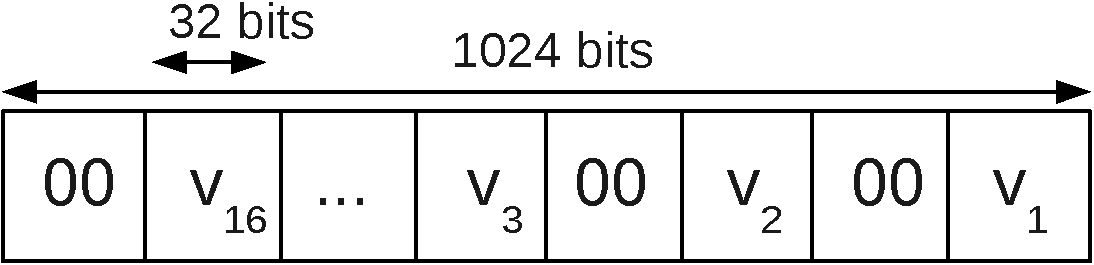
\includegraphics[width=2.0in]{fig/pack.pdf}
\caption{Packing of 16 integer values (32 bits each) into a
	 single 1024-bit value that is subsequently encrypted
	 using $\HOM$.}
\label{fig:pack}
\end{figure}

\textbf{Word search} ($\SEARCH$)\@.  To allow word searches (e.g., using the
``ILIKE'' keyword), we implement a cryptographic protocol for keyword
searches on encrypted text~\cite{Dawn-Song-Search-2000,
amanatidis-boldyreva-o'neill}.  $\SEARCH$ allows the server to detect
repeating words in a given column.


\textbf{Join} ($\JOIN$ and $\OPEJOIN$)\@. 
A separate encryption level is necessary to allow equality joins between
two columns, because the $\DET$ encryption level uses different keys for
each column.  At a high level, $\JOIN$ allows the server
to compare values between values in columns $A$ and $B$, given a token
from the frontend for columns $A$ and $B$\@.  $\JOIN$ also
supports all operations allowed by $\DET$ and $\SEARCH$, and also allows
the server to detect repeating values between two columns.
For inequality joins, $\OPEJOIN$ allows the server to perform inequality
joins on any columns at that encryption level.
The mechanics of these encryption levels are discussed in more detail
in \S\ref{ss:join}, along with the entire join mechanism.



\begin{figure}[t!] \centering 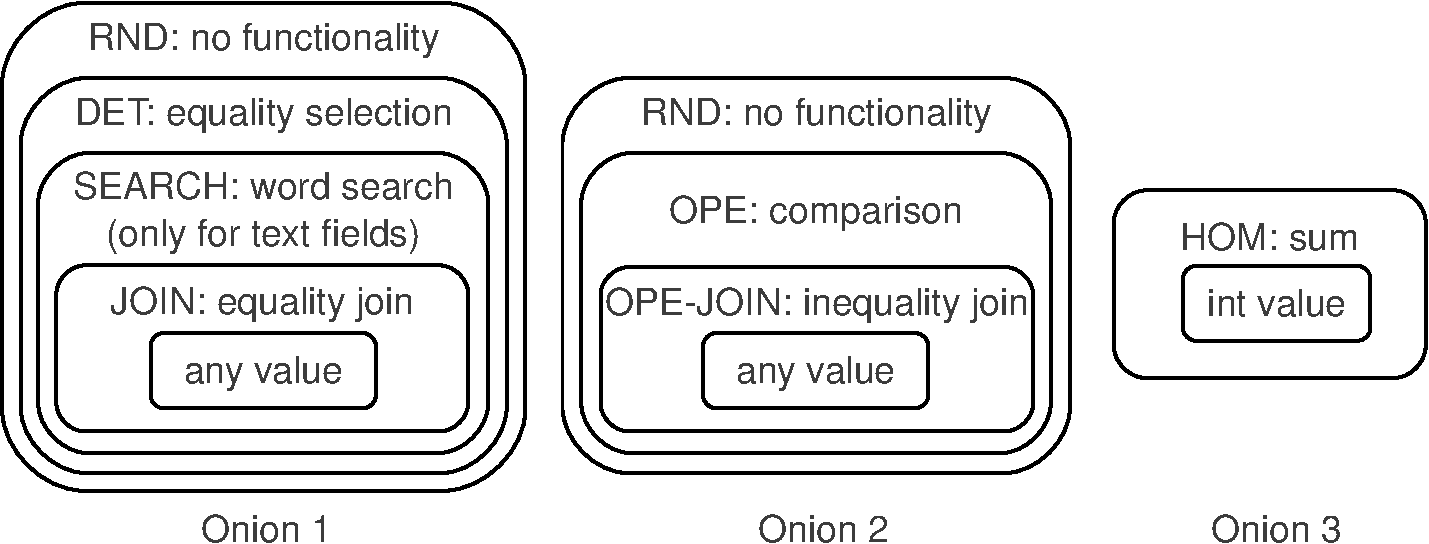
\includegraphics[width=3.3in]{fig/storage.pdf}
\caption{Onion layers of encryption and the classes of computation they allow.}
\label{fig:onion}
\end{figure}

\subsection{Adjustable Query-based Encryption}

A key part of CryptDB's design is \textit{adjustable query-based encryption},
which dynamically determines the level of encryption to reveal to the server.
The answer depends on the queries being asked over the data:
if there is no reason to compare data items in a column or sort a
column, the column will be encrypted with $\RND$, and for columns
that perform equality checks but not inequality checks, $\DET$ suffices.
Unfortunately, there are many databases where the query set
is not known in advance.
Thus, we need an adaptive scheme that dynamically ``does the right thing''
in terms of choosing an encryption strategy for the query at hand.

Our idea is to encrypt each cell independently into an \textit{onion}:
each value in the table is dressed in layers of increasingly stronger
encryption, as illustrated in Figure~\ref{fig:onion}. Each layer of
each onion enables certain kinds of functionality as explained in the
previous subsection.  For example, the outermost layers, $\RND$ and
$\HOM$, provide maximum privacy, whereas $\OPE$ provides more
functionality.  For numeric values, CryptDB maintains three onions,
whereas for string values, CryptDB maintains two onions (i.e.,
no $\HOM$)\@.  To prevent the server from learning information from
column or table names, CryptDB's frontend also anonymizes the schema.
Figure~\ref{fig:schema} shows an example server-side schema and data
under CryptDB, along with the corresponding plaintexts.  Each data
item is stored encrypted in at most 3 onions (for integers) or 2
onions (for non-integer values), although CryptDB's optimizations
can reduce that to 1 onion for some sets of queries (as discussed
in \S\ref{ss:optimize}).

For each level of each onion, the frontend uses the same key for
encrypting values in the same column, and different keys across
columns, onion levels, and tables.  All these keys are derived
from the master key $\MK$\@.  For example, for table $t$, column
$c$, encryption level $l$, the frontend uses the key
\begin{equation}\label{eq:columnkey}
K_{t, c, l} = \mathsf{PRP}_{\MK} (\text{``table $t$'', ``column $c$'', ``level
$l$''}),
\end{equation}
where $\mathsf{PRP}$ is a pseudorandom permutation (such as AES).

Each onion starts out encrypted with the most private encryption scheme
($\RND$ for onions 1 and 2, and $\HOM$ for onion 3)\@.  As the frontend
receives SQL queries from the
application, the onion key manager (OKM) determines whether layers of
encryption need to be removed.  Given a predicate $P$ on column $c$
needed for the query, the OKM first establishes what onion layer is
needed to perform $P$ on $c$.  If the encryption of $c$ is already at
an onion layer that allows $P$, the OKM does nothing.  Otherwise,
the OKM must strip off the onion layers to allow $P$ on $c$, by
sending the corresponding onion key to the server.

To avoid changing the DBMS, CryptDB implements onion layer decryption
using user-defined functions in the server.  For example, to decrypt
onion 2 of column 2 in table 1 to level $\OPE$, the OKM issues the
following query to the server, using the {\tt DECRYPT\_RND} UDF:

\begin{verbatim}
 UPDATE Table1 SET C2-Onion2 =
                   DECRYPT_RND(K, C2-Onion2)
\end{verbatim}
 
\noindent where $K$ is the appropriate key computed as in Eq.
(\ref{eq:columnkey}).

Note that decryption is performed entirely by the server and not by the client.
More importantly, in the steady state, no server-side decryptions are needed,
since column decryption happens only when a new type of predicate is performed
on a column.  For example, after an equality predicate is performed on a column
and the server brings the column to level DET, the column remains in that state,
and future such queries no longer require decryption.  As \S\ref{s:eval}
will illustrate, this ensures that, in the steady state, the overhead of CryptDB
is acceptably low.  The resulting privacy level to which the database converges
is the maximum privacy level for the set of queries issued by the application.



\begin{figure}[t!] 
\centering
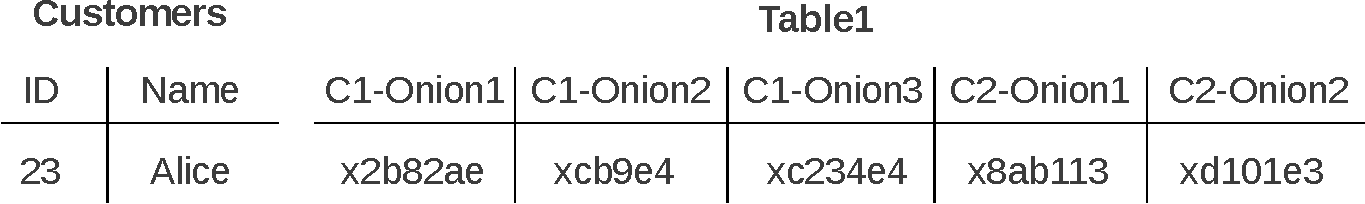
\includegraphics[width=3.4in]{fig/schema.pdf}
\caption{Data layout at the server. When the frontend creates a table
with the schema on the left, the table created at the server is the one from
the right.}
\label{fig:schema}
\end{figure}


\subsection{Query Execution for Read Queries}

To execute each SQL query, the frontend anonymizes, encrypts and rewrites
the query before forwarding it to the untrusted DBMS server.  To anonymize
a query, the frontend replaces each table with the table name from the
anonymized schema (see Figure \ref{fig:schema}).  For projection, the
frontend replaces each column with the name of the anonymized column for
the first onion.  For executing predicates or aggregates on a column, the
frontend replaces the column with the anonymized name of the onion that
allows the necessary operation on that field, and, for certain operations
(such as {\tt SUM}), the frontend replaces the operation with its equivalent
UDF that operates on ciphertexts.
Finally, each constant in the query is encrypted with the encryption scheme
corresponding to the layer of the onion used by the predicate involving the
constant.

To illustrate how this works, consider an example scenario consisting of a
table \texttt{Employees}, which has four columns of interest: \texttt{id},
\texttt{name}, \texttt{address}, and {\tt salary}.
Initially, each column in the table is dressed in all onions of encryption
with $\RND$ and $\HOM$ as outermost layers, as shown in Figure~\ref{fig:onion}.
At this point, the server can learn nothing about the data content other
than the number of columns, rows, and data size.

To illustrate when onion layers are removed, consider the query
\texttt{SELECT * FROM Employees WHERE name = 'Alice'},
which requires lowering encryption of {\tt name} to level $\DET$\@.
In this case, the frontend first issues the query
\texttt{UPDATE Table1 SET C2-Onion1 = DECRYPT\_RND($K_{1,2,\RND}$,
C2-Onion1)}, and then 
\texttt{SELECT C1-Onion1, C2-Onion1, C3-Onion1, C4-Onion1 FROM Table1
WHERE C2-Onion1 = x7d35a3}, where  
\texttt{x7d35a3} is an encryption of ``Alice'' with key $K_{1,2,\DET}$\@.
The frontend decrypts the results from the server and returns them to
the user.

If the next query is {\tt SELECT COUNT(*) FROM Employees WHERE
name = 'Bob'}, no additional server-side decryptions are necessary, and
the frontend directly issues the query {\tt SELECT COUNT(*) FROM Table1
WHERE C2-Onion1 = xbb234a}, where x$bb234a$ is the encryption of ``Bob''.

Finally, the frontend replaces aggregation operators with
equivalent UDFs that operate on encrypted values.  For example,
if the user issues the query {\tt SELECT SUM(salary) FROM Employees},
the frontend rewrites it to {\tt SELECT HOM\_AGG(C4-Onion3,
PKTABLE.PK) FROM Table2}, where {\tt HOM\_AGG} is a UDF that performs
Paillier multiplication (resulting in addition of plaintexts),
{\tt PKTABLE} is a table of public keys \name{} stores at the server
(see Fig.~\ref{fig:architecture}), and $\PK$ is the Paillier public
key modulus.


\subsection{Query Execution for Write Queries}

CryptDB also supports queries that modify data on the server---namely,
{\tt INSERT}, {\tt DELETE}, and {\tt UPDATE}.  For all modification queries,
the frontend applies the same processing to the predicates (i.e., the
{\tt WHERE} clause) as for read queries.  For {\tt INSERT} queries, the
frontend encrypts each inserted column's value with each onion layer
that has not been stripped off yet in that column.  For {\tt DELETE}
queries, no additional processing is performed.  For {\tt UPDATE}
queries that set the value of a column to a constant, the frontend
encrypts the value in the appropriate onions as for {\tt INSERT}.

The remaining case is {\tt UPDATE} queries that update a column value
based on another column value, such as {\tt salary=salary+1}.
Such an update would have to be performed using $\HOM$, because it
allows additions.  However, in doing so, the values in the $\OPE$ and
$\DET$ onions would become stale.  In fact, an encryption scheme that
allows both addition and comparison at the same time is fundamentally
insecure: if a malicious server knows the order of the items ($\OPE$)
and can increment the value by one, the server can keep adding one to
each field homomorphically until the field becomes equal to some other
value.  This would allow the server to compute the difference between
any two values in the database, which is almost equivalent to knowing
their values. 

There are two solutions to this problem.
If a column is incremented and then only projected (no comparisons
performed on it), the solution is simple: when requesting the value
of this field, use the value of Onion 3 rather than Onion 1 or 2,
because Onion 3 is up-to-date.
This is the case for most TPC-C queries.
If a column is used in comparisons after it is incremented, the
solution is to split the query into two.
That is, for query \texttt{UPDATE Employees SET salary=salary+1
WHERE id=3}, the frontend issues the encrypted version of
\texttt{SELECT salary FROM Employees WHERE id=3}, and then
the encrypted version of
\texttt{UPDATE Employees SET salary=z WHERE id=3}, where
$z$ is one more than the result of the first
query.\footnote{If the first {\tt SELECT} query returns more than
one result, the frontend computes a mapping of old encrypted
{\tt salary} values and the corresponding new encrypted {\tt salary}
values, and uses a UDF in the second {\tt UPDATE} query to update
the {\tt salary} column according to this mapping.}
However, in most cases in practice (such as in TPC-C), such updates
are executed on individual rows.

\subsection{Computing Joins}
\label{ss:join}
 
Supporting joins is a challenging problem.  If two columns are to be
joined, they need to be encrypted with the same key for levels
$\JOIN$ or $\OPEJOIN$.  We first describe how CryptDB implements
deterministic joins (the overwhelmingly common case, i.e., level
$\JOIN$), and then describe inequality joins (level $\OPEJOIN$).

To provide maximum privacy for equality joins, the server should not
be able to join columns for which the user did not request a join,
so columns that are never joined should not be encrypted with the
same cryptographic $\JOIN$ keys.  Moreover, if users request a join
of columns
$A$ and $B$, and a join of columns $C$ and $D$, the server should
not be able to join $B$ and $C$\@.  Thus, the question is, which
$\JOIN$ keys should each column be encrypted with, given that we
do not know in advance what columns will be joined?

To address this problem, we propose a new cryptographic primitive that
allows the server to dynamically adjust the $\JOIN$ encryption keys
of each column.  Each column is initially encrypted with a different
$\JOIN$ key, thus disallowing all joins.  When the user requests a
join, the frontend will give the server an onion key to re-encrypt
the two columns to the same $\JOIN$ key, allowing joins between the
two columns.

Our algorithm is based on elliptic-curve cryptography (ECC).  When
a row is initially inserted, the $\JOIN$ encryption of value $v$
is computed as $\JOIN_K(v) := H(v)^K$, where $K$ is the initial key
for that table, column, and level, and $H$ is a mapping from values
(integers or strings) to an elliptic curve.  When the user requests
to join columns $c$ and $c'$, the frontend computes $\Delta K=K/K'$,
which can be used to bring the $\JOIN$ encryptions of $c$ and $c'$
to the same key.  Given $\JOIN_{K'}(v)$ (stored in column $c'$) and
$\Delta K$, the server uses a UDF to compute $\JOIN_{K'}(v)^{\Delta
K} = H(v)^{K'\times K / K'} = H(v)^K = \JOIN_K(v)$.  Now that columns
$c$ and $c'$ share the same $\JOIN$ key, the server can perform an
equality join on $c$ and $c'$ as usual.

\begin{theorem}
The server can only join pairs of columns that were joined by
a legitimate user query.
\end{theorem}

\begin{proof}[sketch]
We delegate the full proof to the extended version of this paper,
and provide only a sketch here.
Our scheme is secure (i.e., the theorem is true) because $K/K'$ does not reveal any
information about $K$ or $K'$ alone.  Moreover, the server cannot compute
$K$ from $H(v)^K$ because of the hardness assumption of computing the
discrete logarithm in elliptic curve-based groups. Given two columns
encrypted with $K$ and $K'$, if the server is not given $K/K'$, it
cannot bring the two columns to the same encryption level, and thus
cannot perform unrequested joins.
\end{proof}

We chose ECC because of its efficiency: computing $\JOIN_{K'}(v)^{K/K'}$
is basically a multiplication, and does not involve any exponentiations.
Moreover, elliptic curve-based ciphertexts are small ($\approx 160$ bits)
compared to ciphertexts in typical public key cryptosystems for the same
security level~\cite{nsaecc}.

For inequality joins, a similar dynamic re-encryption scheme is difficult
to construct.  Instead, CryptDB requires that pairs of columns that will
be involved in inequality joins are declared by applications ahead of
time, by annotating the schema, so that matching keys are used for level
$\OPEJOIN$ of those columns.  Alternatively, level $\OPEJOIN$ encryptions
can be re-encrypted with matching keys at the expense of sending an entire
column to the frontend for re-encryption, and then sending it back
to the DBMS server.


\subsection{Transactions and Indexes}

CryptDB uses existing transaction and indexing mechanisms in the
DBMS server without any modifications.  For transactions, the
frontend passes along any {\tt BEGIN}, {\tt COMMIT}, and
{\tt ABORT} queries to the DBMS, and CryptDB does not change any
transaction semantics.  For indexes, the DBMS builds indexes
of encrypted columns much the same way in which it builds
indexes of plaintext data.  The frontend does not request
indexes on $\RND$ encryptions, since no lookups are performed
at that level, but the frontend does construct indexes on
$\DET$, $\JOIN$, $\OPE$, and $\OPEJOIN$ encryptions, if the
application requested an index on the corresponding column
in the original schema (e.g., using an {\tt ALTER} or {\tt CREATE}
query).


\subsection{Optimizations}
\label{ss:optimize}

CryptDB implements three important optimizations to improve
its performance, which we now describe.

\textbf{Known query set.}  For many applications, the queries issued
by the application are fixed and known ahead of time.  In this case, we
do not need to adjust onion levels at runtime, and can start the database
with the exact onion encryption levels that we need.  Moreover, if a
certain column is never used in certain operations, the corresponding
onion can be omitted altogether.  For example, if an application never
performs range or order operations on a column, the $\OPE$ onion for
that column can be omitted.  Discarding onions significantly reduces
performance costs both in the frontend and in the DBMS server.  This
optimization is implemented by a \textit{train} module in the frontend,
which, given a set of queries a user application will issue, determines
the exact levels of encryption needed.

\textbf{Security convergence.}  Even if the query set is not known in
advance, after an application has run for a considerable while on a DB,
the frontend may drop any onions that have not been used, because these
onions are unlikely to be used in the future.  If a query does happen
to use these onions later, the frontend can go through the cost of
inserting the deleted column, by downloading the entire column and
re-uploading it in a different, re-encrypted onion.  Since these
operations are amortized over long periods of time, the overall
performance remains high.

\textbf{Ciphertext caching.}  A significant ongoing cost for the
frontend lies in generating $\OPE$ and $\HOM$ encryptions of
constants used in queries.  To avoid this cost, the frontend
maintains a cache of recently-used constants, along with their
encryptions under different keys.  Since some constants are
repeatedly used in many queries (e.g., the constant $1$),
this optimization reduces the amount of CPU time spent by
the frontend encrypting data.


\subsection{Discussion and Limitations}

CryptDB's design supports most relational queries and aggregates
on standard data types, such as integers and text/varchar types.
Numeric data of decimal type with $p$ digits after the decimal
can be mapped to integer types by multiplying the input by $10^p$.
CryptDB can encrypt floating-point values, but cannot perform
aggregations on floating-point values per se (however, if the
values are converted to fixed-point, CryptDB can use $\HOM$
for aggregation).
Additional operations can be added to CryptDB by extending its
existing onions, or adding new onions for specific data types.
For example, one could add spatial and multi-dimensional range
queries using the protocols proposed by Shi et al~\cite{multidimRangeQueries}.

CryptDB has certain limitations.  For example, it does not support
both computation and comparison {\em in the same predicate},
such as \texttt{WHERE salary > age*2+10}.
CryptDB can facilitate processing such a query, but it would require
a little bit of processing on the frontend.
To use CryptDB, the query can be rewritten into a sub-query that
selects a whole column, \texttt{SELECT age*2+10 FROM $\ldots$},
which CryptDB computes using $\HOM$, then re-encrypting the
results in the frontend, creating a new column (call it {\tt aux})
at the server consisting of the newly-encrypted values, and finally
running the original query with the predicate {\tt WHERE salary > aux}.

The current CryptDB prototype does not support stored procedures or
other user-defined functions on the server.  Supporting stored
procedures written in SQL should be straightforward, by having the
frontend rewrite the SQL statements inside of the stored procedure
as it would for any other query.  On the other hand, CryptDB's
design cannot support the execution of arbitrary user-defined
functions (not written in SQL) over encrypted data.

Finally, our current prototype handles server-side auto-increment
columns by leaving the column values in plaintext on the server.
We believe this is an acceptable trade-off, since the server is
anyway involved in choosing the auto-incremented value.  A more
privacy-preserving scheme may involve using $\HOM$ to generate
the auto-incremented value, but $\HOM$ would not allow joins on
that column (whereas auto-increment is commonly used for primary
key columns that require joins).  More generally, CryptDB allows
columns that are not privacy-sensitive to be left unencrypted
on the server, to reduce overhead and allow more general
computations (such as arbitrary UDFs).


% \subsection{Access Control}
% 
% Access control can be implemented at the frontend or at a machine between the
% users and the front end. There has been significant work done on such schemes
% which can be used with CryptDB\@. 



\section{Privacy Analysis}
\label{s:analysis}

In this section, we prove that CryptDB achieves the privacy goal we set
out in \S\ref{s:model}.  To do so, we assume that the cryptographic tools
used by CryptDB actually provide the properties we require.  The constructions
we proposed as implementations in the previous section are secure based on
some cryptographic assumptions; if such assumptions are ever broken, the
cryptographic constructions can be replaced by others that have the same
security guarantees, thus preserving the security of the overall CryptDB
design.

\begin{theorem}
The server in CryptDB learns as much
information about the data in the database as does the server in the Ideal
System from Definition~\ref{def:sec}.
\end{theorem}

\begin{proof}[sketch]
The proof is by induction on
the queries requested. The base case of the
induction is when no queries have been requested so far. Since we start out the
database with $\RND$, we satisfy the base case. 

In the inductive
step, we need to prove that, by processing the $i^\mathrm{th}$ query, $Q_i$, the server
only learns as much information as the relations contained in $\fu(Q_i)$. Such proof is by
exhaustively considering all types of operations; for
brevity, we only consider the most basic ones here, leaving the remainder for
the extended version of this paper.
Suppose $Q_i$ contains an equality predicate:
\texttt{c1 = x1c5a21}. Then,  $\fu(Q_i)$ contains the relation \{\texttt{c1 =
*}\}. CryptDB will lower the level of {\tt c1} to $\DET$\@.
By assumption about the security level provided by $\DET$, the server
can only check whether some encrypted data from {\tt c1} equals some
other encrypted data from {\tt c1}, all of which is already permitted by
\texttt{c1 = *} from $\fu(Q_i)$ because the server can replace $*$ with any
value from {\tt c1}.

Now consider that $Q_i$ contains an inequality check \texttt{c1 > x1c5a21},
which means that $\fu(Q_i)$ contains \texttt{\{c1 > *\}}. In this case, CryptDB
will reveal the $\OPE$ encryptions of column {\tt c1} to the server.  By assumption,
$\OPE$ only leaks order between items, that is, {\tt item i $\stackrel{?}{>}$
item j}.  However, this information is already permitted by $\fu(Q_i)$ because
the server can replace {\tt c1} with item $i$ and $*$ with a value from item
$j$ in when posing a question to the oracle from the set of questions allowed by
\{{\tt c1 > *}\}. 
\end{proof}

